%----------------------------------------------------------------------------------------
% Preambulo y Configuración
%----------------------------------------------------------------------------------------

\documentclass[
    11pt,
    spanish,
    singlespacing,
    parskip,
    headsepline,
    bookmarks=true,
    unicode=true,
    pdftoolbar=true,
    pdfmenubar=true,
    pdffitwindow=false,
    colorlinks=true,
    linkcolor=blue,
    citecolor=blue,
    urlcolor=blue
]{MastersDoctoralThesis}

\usepackage[utf8]{inputenc} % Codificación de entrada UTF-8
\usepackage[T1]{fontenc}    % Codificación de salida para caracteres especiales
\usepackage{graphicx}       % Manejo de gráficos
\usepackage{eso-pic}        % Permite agregar fondos
\usepackage{hyperref}       % Manejo de hipervínculos y marcadores

% Redefinición de caracteres problemáticos en marcadores
\hypersetup{
    pdftitle={Título del Documento},
    pdfauthor={Autor del Documento},
    pdfkeywords={Sistemas Embebidos, Internet de las Cosas, Inteligencia Artificial},
    pdfstartview={FitH},
    unicode=true,
    colorlinks=true,
    linkcolor=blue,
    citecolor=blue,
    urlcolor=blue
}

\pdfstringdefDisableCommands{%
  \def\texttt#1{#1}%
  \def\textbf#1{#1}%
  \def\textit#1{#1}%
  \def\"{\"}%
  \def\~{~}%
  \def\'{'}%
  \def\^{}%
  \def\textunderscore{\_} % Manejo del subrayado en marcadores
}


% Definir comandos requeridos por la clase
\newcommand{\degreename}{Maestría en Ciencias} % Cambia según tu título
\newcommand{\univname}{Universidad Nacional de Ejemplo} % Cambia según tu universidad
\newcommand{\keywordnames}{Palabras clave:}
%----------------------------------------------------------------------------------------
% Documento Principal
%----------------------------------------------------------------------------------------

\begin{document}

% Configuración de la portada
\posgrado{Carrera / Maestría}
\keywords{Sistemas Embebidos, Internet de las Cosas, Inteligencia Artificial}

% Incluir la portada desde un archivo separado
%----------------------------------------------------------------------------------------
% PORTADA
%----------------------------------------------------------------------------------------
\begin{titlepage}
    % Fondo completo con el PDF que incluye la barra y el logo
    \AddToShipoutPictureBG*{
\includegraphics[width=\paperwidth, height=\paperheight]{Figures/fondo.pdf}}

    % Contenido principal
    \begin{flushright}
        \setlength{\rightskip}{-2cm} % Ajusta la sangría derecha
        \vspace*{7.5cm} % Ajustar según la posición vertical deseada

        % Título
        {\fontfamily{phv}\bfseries\fontsize{33pt}{40pt}\selectfont
        Título del trabajo} \\[1.5cm]

        % Autor
        {\fontfamily{phv}\fontsize{20pt}{25pt}\selectfont
        Nombre del autor} \\[1cm]

        % Carrera o Maestría (comentar o descomentar la línea correspondiente)
        {\fontfamily{phv}\fontsize{15pt}{20pt}\selectfont
        \textbf{Carrera de Especialización en Sistemas Embebidos}
        % \textbf{Carrera de Especialización en Internet de las Cosas} \\
        % \textbf{Carrera de Especialización en Inteligencia Artificial} \\
        % \textbf{Maestría en Sistemas Embebidos} \\
        % \textbf{Maestría en Internet de las Cosas} \\
        % \textbf{Maestría en Inteligencia Artificial Embebida} \\
        % \textbf{Maestría en Computación de Borde} \\
        % \textbf{Maestría en Inteligencia Artificial} \\
        } \\[2cm]

        % Director
        {\fontfamily{phv}\fontsize{11pt}{15pt}\selectfont
        \textbf{Director:} Director (pertenencia)} \\[1cm]

        % Jurados
        {\fontfamily{phv}\fontsize{11pt}{15pt}\selectfont
        \textbf{Jurados:}} \\[0.5cm]
        {\fontfamily{phv}\fontsize{11pt}{15pt}\selectfont
        Jurado 1 (pertenencia)} \\ 
        {\fontfamily{phv}\fontsize{11pt}{15pt}\selectfont
        Jurado 2 (pertenencia)} \\ 
        {\fontfamily{phv}\fontsize{11pt}{15pt}\selectfont
        Jurado 3 (pertenencia)} \\[2cm]

        % Fecha y lugar
        {\fontfamily{phv}\itshape\fontsize{10pt}{12pt}\selectfont
        Ciudad de [lugar], [mes] de [año]} % Ejemplo: Ciudad de Córdoba, junio de 2025
    \end{flushright}
\end{titlepage}


% Configuración del contenido preliminar
\frontmatter % Usar numeración romana para las páginas preliminares
\pagestyle{plain} % Estilo de encabezado simple

%----------------------------------------------------------------------------------------
% Resumen
%----------------------------------------------------------------------------------------

\begin{abstract}
\addchaptertocentry{\abstractname} % Agregar resumen al índice
El resumen debe escribirse en uno o dos párrafos. Debe ser breve y conciso, sin ningún elemento de formato en el texto como itálicas o negritas. Tampoco se deben usar siglas ni acrónimos que no resulten obvios para un lector promedio de la memoria, ni referencias bibliográficas o notas al pie de página. No debe faltar qué es lo que se hizo/logró, qué importancia/valor tiene el proyecto/resultado, qué va a encontrar el lector en la memoria y qué contenidos de la especialización/maestría se aplicaron en el proyecto.
\end{abstract}

%----------------------------------------------------------------------------------------
% Agradecimientos
%----------------------------------------------------------------------------------------

\begin{acknowledgements}
\vspace{1.5cm}
Esta sección es para agradecimientos personales y es totalmente \textbf{OPCIONAL}.
\end{acknowledgements}

%----------------------------------------------------------------------------------------
% Índice
%----------------------------------------------------------------------------------------

\tableofcontents
\listoffigures
\listoftables

%----------------------------------------------------------------------------------------
% Dedicatoria
%----------------------------------------------------------------------------------------

\dedicatory{\textbf{Dedicado a... [OPCIONAL]}}

%----------------------------------------------------------------------------------------
% Capítulos
%----------------------------------------------------------------------------------------

\mainmatter % Iniciar numeración numérica para el contenido principal
\pagestyle{thesis} % Estilo de encabezado de tesis

% Incluir capítulos desde archivos separados
% Chapter 1

\chapter{Introducción general} % Main chapter title

\label{Chapter1} % For referencing the chapter elsewhere, use \ref{Chapter1} 
\label{IntroGeneral}

En este capítulo se realiza una breve introducción a la necesidad que condujo al desarrollo del trabajo. Se presenta a los sistemas embebidos, la inteligencia artificial y el estado del arte de dispositivos similares. Asimismo, se explica el objetivo y los alcances del trabajo.

%----------------------------------------------------------------------------------------

% Define some commands to keep the formatting separated from the content 
\newcommand{\keyword}[1]{\textbf{#1}}
\newcommand{\tabhead}[1]{\textbf{#1}}
\newcommand{\code}[1]{\texttt{#1}}
\newcommand{\file}[1]{\texttt{\bfseries#1}}
\newcommand{\option}[1]{\texttt{\itshape#1}}
\newcommand{\grados}{$^{\circ}$}

%----------------------------------------------------------------------------------------

%\section{Introducción}

%----------------------------------------------------------------------------------------
\section{La inteligencia artificial y los sistemas embebidos en la agricultura}

En las últimas décadas, la cosecha de frutos ha experimentado un notable proceso de transformación, impulsado por la integración de tecnologías como los sistemas embebidos y la inteligencia artificial. Estos sistemas, capaces de realizar tareas específicas en tiempo real, se han vuelto fundamentales en la modernización de este sector.

Por otra parte, una de las actividades clave consiste en estimar, lo más exactamente posible, la producción total, ya que esto condiciona un conjunto importante de aspectos logísticos que deben ser atendidos correctamente durante la recolección.

Actualmente, el volumen de cosecha se estima al contar los frutos por unidad de superficie en una etapa avanzada de desarrollo. Sin embargo, esta evaluación tardía es demasiado cercana a la cosecha y muy dificultosa en plantaciones medianas o grandes.

Es en este contexto, el prototipo desarrollado permite recolectar imágenes de la plantación con el fin de realizar una detección de objetos. De esta forma, se obtiene una estimación de los frutos para facilitar la toma de decisiones operativas y estratégicas \citep{Mendoza2021}.





\subsection{Especificaciones funcionales del prototipo}
\label{requerimientos_del_sistema}

Se detallan los requerimientos del prototipo, con las funcionalidades y características implementadas.

\begin{enumerate}
	\item Funcionalidades principales del sistema:
		\begin{enumerate}
			\item El sistema registró la temperatura del ambiente.
			\item El sistema registró la humedad del ambiente.
			\item El sistema informó el espacio disponible en la tarjeta microSD.
            \item El sistema informó la cantidad de fotografías almacenadas.
            \item El sistema detectó los frutos en las imágenes capturadas.
            \item El sistema informó el volumen estimado de cosecha.
		\end{enumerate}
	\item Características adicionales del sistema:
		\begin{enumerate}
			\item El sistema resultó escalable, lo que permite la incorporación de nuevos sensores en el futuro.
			\item El firmware estuvo modularizado.
            \item El firmware se desarrolló sobre un sistema operativo de tiempo real.
		\end{enumerate}
    \item Funcionalidades de la interfaz gráfica en la pantalla LCD:
		\begin{enumerate}
			\item La pantalla mostró los valores de humedad y temperatura.
			\item La pantalla mostró el espacio disponible en la tarjeta microSD.
            \item La pantalla mostró la cantidad de fotografías almacenadas.
            \item La información en pantalla se actualizó cada 5 segundos.
		\end{enumerate}
    \item Funcionalidades de interoperabilidad:
		\begin{enumerate}
			\item Las fotografías se almacenaron en formato de archivo JPG.
			\item Las imágenes capturadas alcanzaron una resolución mínima de 640 × 480 píxeles.
            \item Cada imagen guardada no superó un tamaño de 10 MB.
		\end{enumerate}
\end{enumerate}

%----------------------------------------------------------------------------------------

\section{Estado del arte}

Durante la etapa de investigación del trabajo, se realizó una búsqueda de productos comerciales en el mercado local e internacional. Se encontraron algunos con características similares al que se pretende desarrollar. Un dato interesante a resaltar es que todos los productos hallados provienen del mercado internacional; no se identificó ningún producto o empresa que ofrezca este tipo de soluciones en el mercado local hasta el momento. A continuación, se describen los hallazgos encontrados.

\subsection{Fruitometry}

La tecnología de estimación digital de cultivos (DCE) de Fruitometry que se muestra en la figura \ref{fig:Fruitometry}, permite a los productores y administradores de huertos observar el desempeño de su cultivo durante la temporada de cosecha. Esto ayuda a maximizar los rendimientos, reducir los costos de cultivo y proporcionar estimaciones antes de la recolección.

Las unidades de campo, montadas en cuatriciclos y vehículos todo terreno, contienen una variedad de cámaras y sensores que capturan información sobre la densidad de cultivos y las características del huerto. Para cada escaneo de la plantación, se toman miles de fotografías. Luego, estas se procesan en tiempo real mediante el motor de inteligencia artificial con aprendizaje profundo para identificar brotes, flores, frutos y características de interés.

Este conjunto de datos se utiliza para crear un mapa de calor de densidad resumido y generar informes que se usan para tomar decisiones sobre cómo mejorar el rendimiento del huerto, identificar áreas que requieren atención y dirigir la mano de obra hacia ellas \citep{WEBSITE:Fruitometry2024}.

\vspace{1cm}
\begin{figure}[htbp]
	\centering
	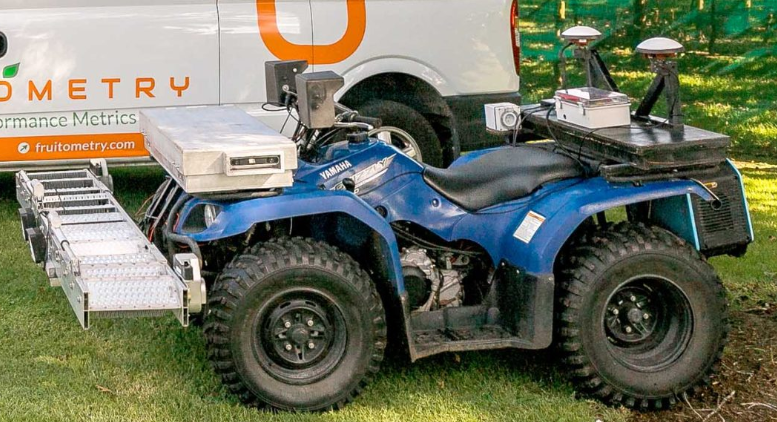
\includegraphics[width=.5\textwidth]{./Figures/Fruitometry.png}
	\caption{Unidad de campo Fruitometry\protect\footnotemark.}
	\label{fig:Fruitometry}
\end{figure}
\vspace{1cm}

\footnotetext{Imagen tomada de \url{https://fruitometry.com/about-fruitometry/}}

\subsection{Detección de frutos en imágenes de campo}

En un trabajo de investigación realizado en la Universidad Yangling, China, se capturaron imágenes de kiwis en un huerto bajo diferentes condiciones de iluminación y en distintos momentos del día: mañana, tarde y noche, tanto con flash como sin él. Estas fotografías fueron empleadas para la detección de objetos mediante un modelo llamado Faster R-CNN, implementado con la arquitectura VGG16. Después de aplicar las detecciones, el modelo alcanzó una precisión promedio del 87,61 \%. En la figura \ref{fig:Song2019} se muestran los resultados obtenidos.

Este sistema de visión artificial resultó ser eficaz en la detección de diferentes categorías de frutos en el campo y actuó como un soporte fundamental al robot cosechador. Equipado con este sistema, el robot operó de manera continua durante la temporada de cosecha, lo que representó un avance significativo hacia la automatización de la recolección agrícola \citep{Song2019}.

\vspace{1cm}

\begin{figure}[htbp]
	\centering
	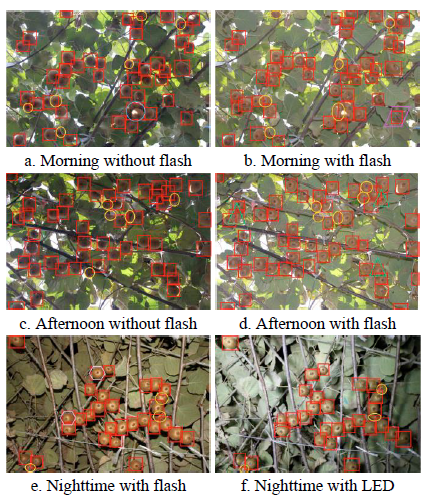
\includegraphics[width=.5\textwidth]{./Figures/Song2019.png}
	\caption{Resultados de una detección de objetos\protect\footnotemark.}
	\label{fig:Song2019}
\end{figure}

\vspace{1cm}
\footnotetext{Imagen tomada de "Kiwifruit detection in field
images using Faster R-CNN with VGG16"}

\newpage
\subsection{Calibrado de frutas}

Existen diversos productos comerciales que aplican la detección de objetos para llevar a cabo procesos de clasificación y calibrado de frutas u hortalizas. Estas máquinas mostradas en la figura \ref{fig:calibrado_de_frutas}, estan diseñadas para grandes cadenas de distribución, automatizan la selección y el empaquetado de los productos, lo que incrementa la eficiencia y reduce los tiempos operativos. El sistema funciona a través de una cinta transportadora equipada con cámaras, que capturan imágenes en tiempo real de cada elemento \citep{WEBSITE:Unitec2024}.

Además de identificar cada objeto, las cámaras registran una serie de parámetros importantes, como el diámetro, la longitud, la forma y, en algunos casos, el color. Estos datos se procesan con algoritmos de visión artificial, que clasifican los productos según criterios preestablecidos de calidad.

\vspace{1cm}
\begin{figure}[htbp]
	\centering
	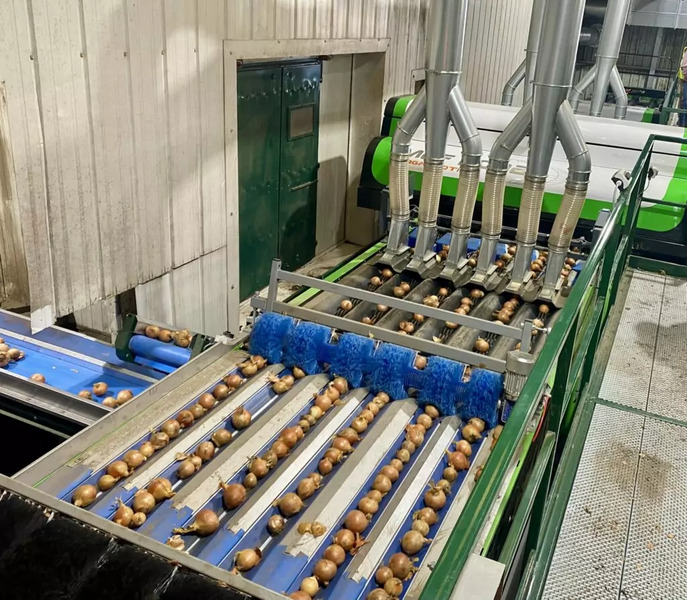
\includegraphics[width=.6\textwidth, height=6cm]{./Figures/calibrado_de_frutas.jpg}
	\caption{Máquina de calibrado de frutas MAF\protect\footnotemark.}
	\label{fig:calibrado_de_frutas}
\end{figure}
\vspace{1cm}

\footnotetext{Imagen tomada de \url{https://tongengineering.com/product/maf-roda-weight-grading/}}

\subsection{Estimación de cosechas mediante imágenes satelitales y drones}

La teledetección se consolidó como una herramienta clave para la estimación de cosechas y el monitoreo de cultivos a gran escala. En la figura \ref{fig:drones_en_cultivos} se muestra el uso de imágenes satelitales de alta resolución, combinadas con sensores multiespectrales y drones equipados con cámaras especializadas, permite la generación de modelos predictivos del rendimiento agrícola. Estos sistemas proporcionan información temprana sobre el estado vegetativo de los cultivos, lo cual facilita la toma de decisiones en diferentes etapas de la producción.

Diversos estudios demostraron que la integración de índices de vegetación, como el NDVI (\textit{Normalized Difference Vegetation Index}), junto con técnicas de aprendizaje automático, ofrecen resultados consistentes en la predicción del volumen de cosecha en plantaciones frutales y agrícolas. A diferencia de los métodos manuales de conteo de frutos, estas tecnologías permiten la evaluación periódica y no invasiva de grandes extensiones de terreno, lo que contribuye a la reducción de costos operativos y a una mayor precisión en la planificación logística.

Por otro lado, la ventaja de estas soluciones radica en su capacidad de escalar desde parcelas individuales hasta áreas regionales, lo que las convierte en una herramienta estratégica para el análisis de la producción agrícola en escenarios de mediana y gran envergadura \citep{Hobart2025}.

\vspace{1cm}
\begin{figure}[htbp]
	\centering
	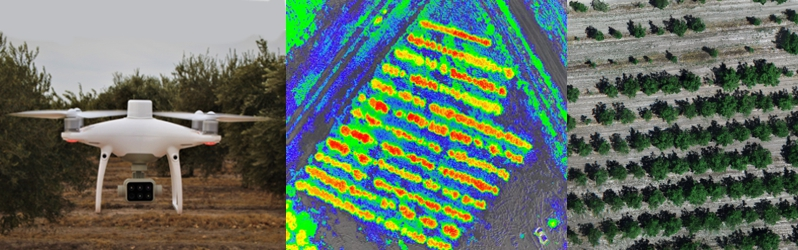
\includegraphics[width=1\textwidth, height=6cm]{./Figures/drones_en_cultivos.jpg}
	\caption{Imágenes tomadas con drones y satélites\protect\footnotemark.}
	\label{fig:drones_en_cultivos}
\end{figure}
\vspace{1cm}

\footnotetext{Imagen tomada de "Monitoreo de cultivos mediante el uso de sensores remotos montados en drones"}

%----------------------------------------------------------------------------------------

\section{Objetivo y alcances}

En la siguiente sección se describen los objetivos del proyecto, los alcances y los aspectos no considerados en el desarrollo del prototipo.

\subsection{Objetivo}

El objetivo del presente trabajo es el desarrollo e implementación de un prototipo que permita contabilizar el rendimiento esperado de un lote de producción de frutos en forma temprana, a través del procesamiento de imágenes.

\subsection{Alcances contemplados}
El alcance establecido para el trabajo incluyó las siguientes tareas:

\begin{itemize}
\item Implementación de un prototipo funcional que toma fotografías de forma automática.
\item Desarrollo del firmware sobre un sistema operativo de tiempo real.
\item Desarrollo del modelo de detección de objetos.
\item Recolección de imágenes para el proceso de entrenamiento.
\item Establecer como fruto objetivo  de detección el kiwi.
\end{itemize}

\subsection{Aspectos no incluidos en el prototipo}
\label{Aspectos_no_incluidos_en_el_prototipo}
El alcance establecido para el trabajo no incluye las siguientes tareas:

\begin{itemize}
\item Pruebas de funcionamiento en la plantación.
\item Desarrollo de la carcasa contenedora del prototipo.
\end{itemize}

%----------------------------------------------------------------------------------------

\chapter{Introducción específica} % Main chapter title

\label{Chapter2}

%----------------------------------------------------------------------------------------
%	SECTION 1
%----------------------------------------------------------------------------------------
En el presente capítulo se describen los componentes de hardware, software y herramientas utilizados para realizar el proyecto.

\section{Estructura del sistema}

En las siguientes secciones se describe la estructura del sistema, con un enfoque en los sistemas embebidos, la detección de objetos y el prototipo desarrollado.

\subsection{Los sistemas embebidos}

En el contexto de la agricultura moderna, los sistemas embebidos se diseñaron para la ejecución de tareas específicas en tiempo real. En el caso del prototipo desarrollado, el sistema se compuso de una serie de módulos, entre ellos cámaras, sensores, pantallas y unidades de almacenamiento. 

Este pudo montarse en un medio de transporte adaptado a las características de la plantación, lo que permitió la captura automatizada de imágenes de los frutos, así como el registro de datos ambientales relevantes durante el recorrido. Toda la información recolectada se almacenó de forma local en una tarjeta microSD, lo que posibilitó su uso de manera independiente de la cobertura de señal.

\subsection{Detección de Objetos}

La detección de objetos constituye una técnica avanzada de visión por computadora que permite identificar y clasificar elementos presentes en las imágenes. Esta tecnología ha demostrado ser particularmente valiosa en el ámbito agrícola, donde la estimación de la producción y la gestión eficiente de los recursos resultan esenciales \citep{Lim2020}.

Para garantizar un funcionamiento correcto de la detección de objetos, se requiere un conjunto de imágenes de entrada. Posteriormente, estas se procesan mediante algoritmos de visión por computadora, que analizan cada entrada con el fin de identificar y contabilizar los frutos \citep{Montiel2019}.

Por otra parte, la detección de objetos se fundamenta en técnicas avanzadas, como el análisis de imágenes y el aprendizaje automático, que permiten diferenciar entre frutos maduros, inmaduros y otros elementos presentes en la plantación.

\newpage

\subsection{El prototipo SIVIC}

El prototipo desarrollado, a partir de ahora denominado SIVIC (Sistema de Visión para Cultivos), está conformado por tres partes esenciales que permiten llevar a cabo su labor. Estas son:
\begin{itemize}
\item El nodo sensor: esta es la parte física o hardware del sistema, utilizado para adquirir las imágenes de la plantación.
\item El firmware: este abarca la lógica del sistema y se encarga de la adquisición, procesamiento y la gestión del almacenamiento de datos. Puede funcionar sobre un sistema operativo de tiempo real o no.
\item El modelo de detección de objetos: este permite realizar la contabilización de los frutos encontrados en las imágenes proporcionadas como entrada.
\end{itemize}

\section{Componentes principales de hardware}

En esta sección se describen en detalle los componentes de hardware y software seleccionados para este trabajo, que resultaron clave para garantizar el funcionamiento de SIVIC.

\subsection{Plataforma de desarrollo STM32 Nucleo-F429ZI}
\label{subsec:F429ZI}

La placa STM32 Nucleo-F429ZI, posee un núcleo ARM Cortex-M4. Esta placa ofrece una plataforma flexible para desarrollar aplicaciones embebidas, con una amplia variedad de interfaces y periféricos, como ADC, DAC, GPIO, SPI, I2C, USART, entre otros. Además, cuenta con compatibilidad con los ecosistemas Arduino y ST Morpho, lo que facilita la expansión y el prototipado rápido. Es ideal para proyectos que requieren procesamiento en tiempo real, gestión de múltiples tareas y alto rendimiento \citep{WEBSITE:Itt2024}.

Características:
\begin{itemize}
\item STM32F429ZIT6 en paquete LQFP144.
\item CPU ARM® Cortex®-M4 de 32 bits con FPU.
\item Frecuencia máxima de CPU de 180 MHz.
\item VDD de 1,8 V a 3,6 V.
\item Flash de 2048 KB.
\item GPIO (114) con capacidad de interrupción externa.
\item Controlador DMA de 16 flujos con FIFO y compatibilidad con ráfagas.
\item USB 2.0 OTG SA.
\item I2C.
\item SPI.
\item USART/UART.
\end{itemize}

\subsection{Sensor de temperatura y humedad DHT11}
\label{subsec:dht11}

Este dispositivo, se utiliza para medir temperatura y humedad en ambientes controlados. Es altamente popular debido a su bajo costo y facilidad de uso. Dispone de un sensor capacitivo para medir la humedad y un termistor para la temperatura. El DHT11 proporciona lecturas de humedad en un rango del 20\% al 90\% con una exactitud de ±5\%, y de temperatura entre 0 °C y 50 °C con una precisión de ±2 °C. Se comunica mediante una señal digital, lo que lo hace ideal para aplicaciones en sistemas embebidos y proyectos medianos \citep{WEBSITE:Dht112024}.

\subsection{Display LCD}
\label{subsec:DisplayLCD}

Esta pantalla, capaz de mostrar hasta 16 caracteres en 2 filas, Se utiliza en proyectos de electrónica y sistemas embebidos debido a su simplicidad y bajo costo. Cada carácter se forma a partir de una matriz de puntos de 5 x 8 píxeles, lo que permite visualizar letras, números y símbolos. El display es compatible con microcontroladores y microprocesadores, y se controla mediante interfaces paralelas o serie. Resulta ideal para mostrar información básica, como datos de sensores, mensajes o indicadores de estado en tiempo real \citep{WEBSITE:lcd2024}.

\subsection{Cámara Ov7670}
\label{subsec:camara}

Este módulo compacto de captura de imágenes, mostrado en la figura \ref{fig:camara2024}, se utiliza en proyectos de visión por computadora y sistemas embebidos. El sensor de imagen CMOS Ov7670 puede capturar imágenes en resolución VGA (640x480) y CIF (352x288), lo que lo hace adecuado para aplicaciones de procesamiento de imágenes, seguimiento de objetos y reconocimiento de patrones. La cámara se conecta a microcontroladores o plataformas de desarrollo como Arduino y STM32 mediante interfaces I2C o SCCB para configuración, y una interfaz de datos paralela para la transferencia de imágenes. Además, el módulo ofrece control automático de exposición, balance de blancos y eliminación de ruido, lo que garantiza imágenes de calidad en diversas condiciones de luz \citep{WEBSITE:camara2024}.

\begin{figure}[htbp]
	\centering
	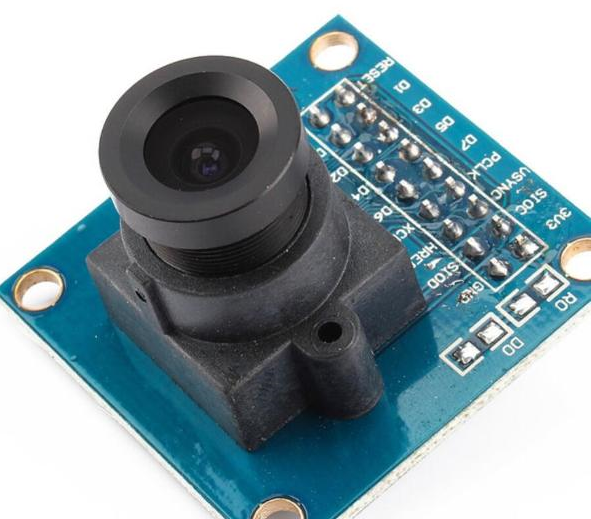
\includegraphics[width=.5\textwidth]{./Figures/camara.png}
	\caption{Cámara Ov7670\protect\footnotemark.}
	\label{fig:camara2024}
\end{figure}

\footnotetext{Imagen tomada de \url{https://www.arcaelectronica.com/products/modulo-de-camara-ov7670-arduino?srsltid=AfmBOopgmnm_0gtPYtNMaSrCGCOKnXMwbjdXpUfh84WJ_Hi9V3akPCPp.}}

\subsection{Sensor ultrasónico HC-SR04}
\label{subsec:hcsr04}

Este dispositivo, mostrado en la figura \ref{fig:hcsr2024}, se utiliza para medir distancias con precisión en proyectos de robótica, sistemas embebidos y automatización. Emite ondas ultrasónicas que se reflejan en objetos cercanos y luego las capta el sensor. El tiempo que tarda la señal en regresar permite calcular la distancia al objeto. El HC-SR04 ofrece un rango de medición de 2 cm a 4 m, con una precisión de aproximadamente 3 mm. Se integra fácilmente con microcontroladores como Arduino o STM32 mediante un sistema de disparo y recepción de señal. Es ideal para aplicaciones como evitar obstáculos, medir niveles de líquido y sistemas de detección de proximidad \citep{WEBSITE:hcsr2024}.

\begin{figure}[htbp]
	\centering
	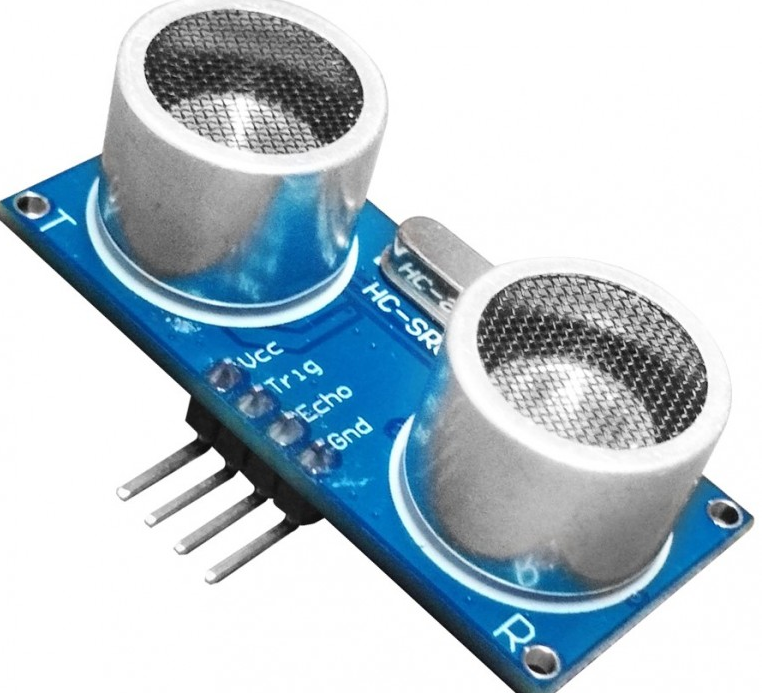
\includegraphics[width=.5\textwidth]{./Figures/hcsr04.png}
	\caption{Sensor ultrasónico HC-SR04\protect\footnotemark.}
	\label{fig:hcsr2024}
\end{figure}

\footnotetext{Imagen tomada de \url{https://www.todomicro.com.ar/modulos/81-sensor-ultrasonico-ultrasonido-hc-sr04-arduino-pic-robotica.html.}}

\section{Herramientas de software y testing utilizados}

Las herramientas de software seleccionadas para este trabajo fueron fundamentales para el desarrollo y las pruebas del prototipo. A continuación se describen en detalle las características principales y los casos de uso de cada una.

\subsection{STM32 CubeIDE}
\label{subsec:stm32}

El sistema STM32 CubeIDE es un entorno de desarrollo integrado (IDE) creado por STMicroelectronics para trabajar con microcontroladores STM32. Basado en Eclipse, STM32 CubeIDE permite a los desarrolladores escribir, compilar y depurar código en lenguajes como C y C++ y por lo tanto facilita el desarrollo de aplicaciones embebidas. También integra herramientas como STM32CubeMX, que configura los periféricos del microcontrolador y genera código automáticamente. Estas  características contribuyen a reducir los errores y a acelerar el proceso de desarrollo. STM32 CubeIDE es compatible con sistemas operativos como Windows, macOS y Linux, y soporta una amplia gama de microcontroladores de la familia STM32, lo que lo convierte en una opción flexible para proyectos de sistemas embebidos \citep{WEBSITE:stm32}.

\subsection{Sistema operativo FreeRTOS}
\label{subsec:FreeRTOS}

Es un sistema operativo en tiempo real (RTOS) de código abierto, ampliamente utilizado en el desarrollo de aplicaciones embebidas. Diseñado para microcontroladores y sistemas de baja potencia, FreeRTOS ofrece un \textit{kernel} ligero y eficiente para gestionar tareas concurrentes de manera óptima. Soporta características clave como multitarea, gestión de memoria, sincronización entre tareas y temporización precisa, lo que lo convierte en una solución ideal para aplicaciones que requieren control preciso del tiempo y recursos limitados.

Además, FreeRTOS es compatible con una amplia variedad de arquitecturas de microcontroladores, incluidos los STM32. Cuenta con una extensa comunidad y soporte comercial a través de \textit{partners} como Amazon Web Services (AWS), que ofrece una versión ampliada llamada FreeRTOS IoT. Gracias a su escalabilidad y flexibilidad, FreeRTOS es una opción popular en proyectos que van desde dispositivos portátiles hasta sistemas industriales complejos \citep{WEBSITE:freertos}.

\subsection{Pruebas en CEEDLING}
\label{subsec:CEEDLING}

Es una herramienta de testing para proyectos en lenguaje C, diseñada para facilitar el desarrollo y la prueba de software embebido. Este marco de pruebas automatizado proporciona un entorno completo para la creación, ejecución y gestión de pruebas unitarias.

Ceedling integra varias herramientas esenciales para el testing, como CMock, un generador de mocks que simula dependencias y facilita el aislamiento de unidades de código durante las pruebas. Además, utiliza Unity, un framework de pruebas unitarias para C, que ofrece una serie de aserciones y macros para verificar el comportamiento del código.

La configuración y ejecución de pruebas con Ceedling se realizan a través de un archivo de configuración, lo que permite una integración fluida en el proceso de desarrollo. La herramienta soporta la ejecución de pruebas en diferentes entornos, genera informes detallados de cobertura de código y facilita la identificación de errores y defectos en el software \citep{WEBSITE:CEEDLING}.

\section{Protocolos de comunicación}

En el diseño de SIVIC, los protocolos de comunicación cumplen un papel esencial en la interacción entre los distintos componentes del sistema. Entre ellos, UART se basa en una comunicación asíncrona, lo que significa que no requiere una señal de reloj compartida entre los dispositivos que se comunican. En su lugar, utiliza parámetros de configuración como la velocidad de transmisión (\textit{baud rate}), la paridad, el número de bits de datos y el número de bits de parada para sincronizar la transmisión y recepción de datos. \citep{WEBSITE:uart}.

I2C, por otra parte, ofrece una solución versátil para la comunicación entre múltiples dispositivos en el sistema. Utiliza dos líneas para la transmisión de datos: la línea de reloj (SCL) y la línea de datos (SDA). La línea SCL sincroniza la comunicación mediante la señal de reloj, mientras que la línea SDA transporta los datos entre los dispositivos conectados. Ambos hilos son bidireccionales, lo que permite que tanto el maestro como el esclavo envíen y reciban información. \citep{WEBSITE:i2c}.

\chapter{Diseño e implementación} % Main chapter title

\label{Chapter3} % Change X to a consecutive number; for referencing this chapter elsewhere, use \ref{ChapterX}

En este capítulo se detallan los problemas encontrados durante el desarrollo del proyecto y los criterios que guiaron la toma de decisiones. Se exponen las justificaciones técnicas y estratégicas de las soluciones implementadas, con un enfoque en cómo cada decisión contribuyó al logro de los objetivos planteados. Además, se incluyen diversos diagramas que contribuyen a ilustrar la arquitectura y el flujo de trabajo del sistema. Este enfoque permite una comprensión integral del proceso de diseño y desarrollo del trabajo realizado.

\definecolor{mygreen}{rgb}{0,0.6,0}
\definecolor{mygray}{rgb}{0.5,0.5,0.5}
\definecolor{mymauve}{rgb}{0.58,0,0.82}

%%%%%%%%%%%%%%%%%%%%%%%%%%%%%%%%%%%%%%%%%%%%%%%%%%%%%%%%%%%%%%%%%%%%%%%%%%%%%
% parámetros para configurar el formato del código en los entornos lstlisting
%%%%%%%%%%%%%%%%%%%%%%%%%%%%%%%%%%%%%%%%%%%%%%%%%%%%%%%%%%%%%%%%%%%%%%%%%%%%%
\lstset{ %
  backgroundcolor=\color{white},   % choose the background color; you must add \usepackage{color} or \usepackage{xcolor}
  basicstyle=\footnotesize,        % the size of the fonts that are used for the code
  breakatwhitespace=false,         % sets if automatic breaks should only happen at whitespace
  breaklines=true,                 % sets automatic line breaking
  captionpos=b,                    % sets the caption-position to bottom
  commentstyle=\color{mygreen},    % comment style
  deletekeywords={...},            % if you want to delete keywords from the given language
  %escapeinside={\%*}{*)},          % if you want to add LaTeX within your code
  %extendedchars=true,              % lets you use non-ASCII characters; for 8-bits encodings only, does not work with UTF-8
  %frame=single,	                % adds a frame around the code
  keepspaces=true,                 % keeps spaces in text, useful for keeping indentation of code (possibly needs columns=flexible)
  keywordstyle=\color{blue},       % keyword style
  language=[ANSI]C,                % the language of the code
  %otherkeywords={*,...},           % if you want to add more keywords to the set
  numbers=left,                    % where to put the line-numbers; possible values are (none, left, right)
  numbersep=5pt,                   % how far the line-numbers are from the code
  numberstyle=\tiny\color{mygray}, % the style that is used for the line-numbers
  rulecolor=\color{black},         % if not set, the frame-color may be changed on line-breaks within not-black text (e.g. comments (green here))
  showspaces=false,                % show spaces everywhere adding particular underscores; it overrides 'showstringspaces'
  showstringspaces=false,          % underline spaces within strings only
  showtabs=false,                  % show tabs within strings adding particular underscores
  stepnumber=1,                    % the step between two line-numbers. If it's 1, each line will be numbered
  stringstyle=\color{mymauve},     % string literal style
  tabsize=2,	                   % sets default tabsize to 2 spaces
  title=\lstname,                  % show the filename of files included with \lstinputlisting; also try caption instead of title
  morecomment=[s]{/*}{*/}
}

%----------------------------------------------------------------------------------------
%	SECTION 1
%----------------------------------------------------------------------------------------
\section{Composición general del sistema}

El prototipo SIVIC se compone de dos partes esenciales que cumplen funciones clave: el nodo sensor y el nodo detector de objetos. A continuación, se describe cada una de estas partes.

\subsection{Diagrama de componentes}

En esta sección, se presenta el diagrama de componentes en la figura \ref{fig:diagrama_de_componentes}. Este diagrama no solo ilustra la estructura general del prototipo, sino también la interacción entre los componentes para cumplir con los objetivos del trabajo.

\vspace{1cm}

\begin{figure}[htbp]
	\centering
	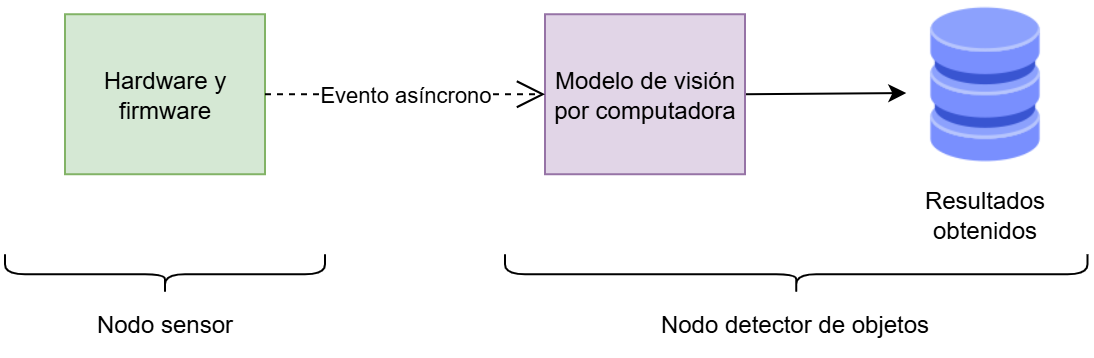
\includegraphics[width=0.8\textwidth, height=0.2\textheight]{./Figures/diagrama_de_componentes.png}
	\caption{Diagrama de componentes.}
	\label{fig:diagrama_de_componentes}
\end{figure}

\vspace{1cm}

El diagrama de componentes ofrece una representación visual clara del sistema SIVIC y facilita la comprensión de cómo las distintas partes se interconectan y colaboran para cumplir con las tareas de detección de frutos. El flujo de información entre el nodo sensor y el nodo detector de objetos establece una secuencia lógica en la que cada componente desempeña un rol clave para el funcionamiento del sistema.



\subsection{El nodo sensor}

El nodo sensor constituye el elemento físico del sistema, encargado de adquirir imágenes de la plantación de manera automatizada. Este se compone de cámaras y otros sensores que recopilan información relevante, como las condiciones ambientales. Estos dispositivos se conectan al sistema para capturar datos visuales y ambientales que serán procesados posteriormente. Su principal función es proporcionar los datos necesarios para la siguiente fase, lo que asegura imágenes de calidad suficiente para permitir la detección de los frutos. A continuación, se describen en detalle los sensores y periféricos seleccionados que forman parte del nodo:

\begin{itemize}
\item La cámara Ov7670 es el elemento central para adquirir imágenes en el sistema. Su elección se basó en la capacidad de la cámara para ajustar automáticamente la exposición y el balance de blancos mantiene una calidad de imagen uniforme, incluso bajo condiciones de iluminación cambiantes. Esta característica es especialmente valiosa en las plantaciones de kiwi, donde la disposición de las hojas genera contrastes y sombras, y la iluminación varía según la hora del día, lo que permite optimizar la calidad de las imágenes obtenidas en diferentes entornos de luz.

\item El sensor de temperatura y humedad DHT11 recopila datos ambientales que complementan la información visual y  permiten obtener un perfil más completo de las condiciones en las que se encuentra la plantación. Estas mediciones pueden ajustarse para optimizar los algoritmos de procesamiento de imágenes y así mejorar la detección de frutos en situaciones adversas.
\item El sensor ultrasónico HC-SR04 se utiliza para asegurar que las imágenes capturadas se realicen a una distancia óptima de los frutos, lo que garantiza que los kiwis ocupen un espacio adecuado dentro del campo de visión de la cámara.
\item La pantalla LCD funciona como una interfaz directa para el usuario en el nodo sensor. Presenta información relevante, como la distancia medida por el sensor ultrasónico, los datos de temperatura y humedad proporcionados por el DHT11, y el estado de las imágenes capturadas por la cámara.
\item El lector de tarjetas SD es crucial para el almacenamiento de las imágenes capturadas y los datos ambientales registrados por los sensores.
\item La placa de desarrollo STM32 Nucleo-F429ZI actúa como el cerebro del nodo sensor. Procesa las señales de los sensores y gestiona la adquisición de datos. La STM32 se comunica con los sensores mediante diversos protocolos, como UART para el sensor ultrasónico e I2C para la pantalla LCD, lo que asegura un funcionamiento coordinado del nodo.
\end{itemize}

El nodo sensor no solo recopila datos visuales y ambientales, sino que también ofrece una interfaz directa para los operadores mediante la pantalla LCD y almacena la información adquirida en el recorrido. Estas funciones permiten que el sistema funcione de manera autónoma, lo que permite el registro de datos valiosos para su análisis posterior. Además, la modularidad del nodo facilita la expansión del sistema en futuras versiones, con la posibilidad de incorporar más sensores o mejorar su capacidad de procesamiento. La figura \ref{fig:nodo_sensor} muestra la composición de este nodo.

\vspace{1cm}

\begin{figure}[htbp]
	\centering
	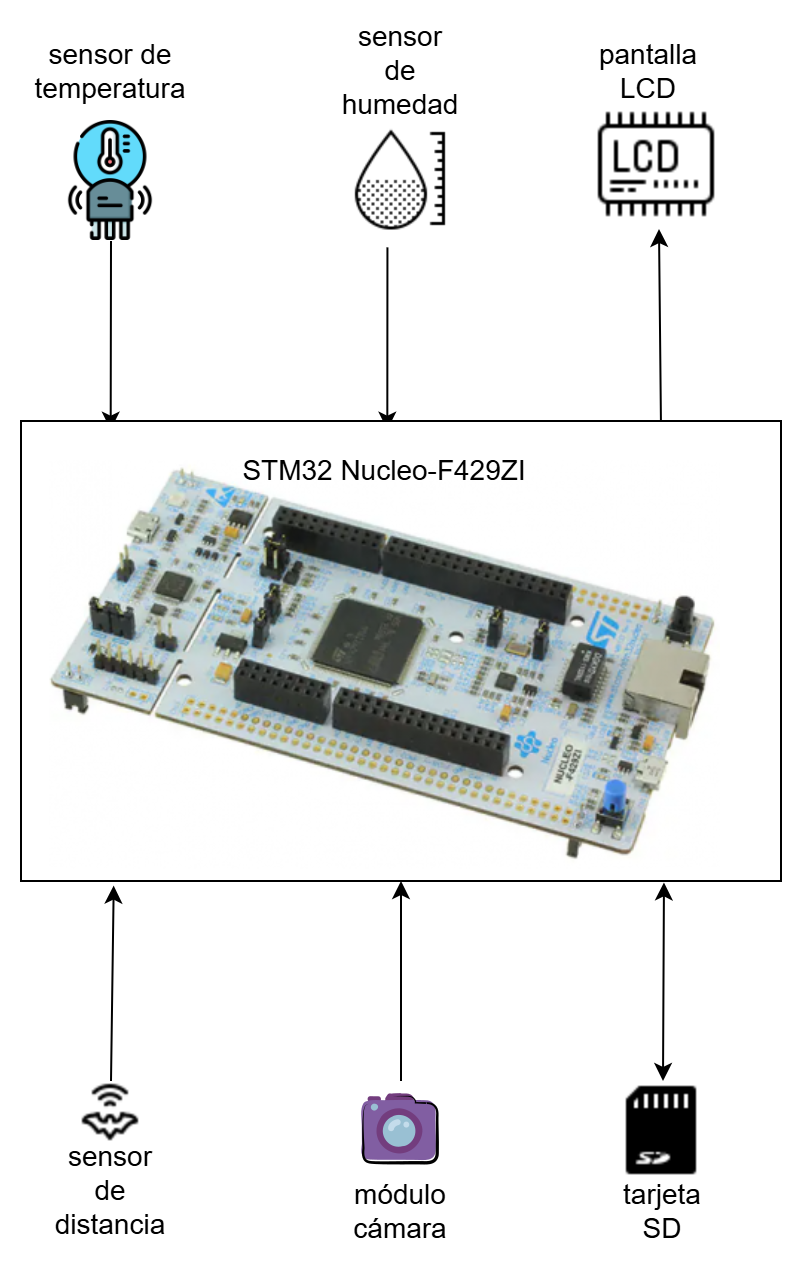
\includegraphics[width=0.6\textwidth, height=0.39\textheight]{./Figures/nodo_sensor.png}
	\caption{Nodo sensor y sus componentes.}
	\label{fig:nodo_sensor}
\end{figure}

\vspace{1cm}

\subsection{El firmware del sistema}

El firmware controla la lógica operativa del sistema y actúa como el vínculo entre los sensores, el procesamiento de datos y el almacenamiento de información. Además, coordina las actividades de los diversos componentes del hardware y ejecuta cada tarea de manera precisa para maximizar la eficiencia operativa del sistema. Su diseño se basa en una estructura por capas que optimiza la organización y legibilidad del código, lo que simplifica la gestión y el mantenimiento de su complejidad. La figura \ref{fig:firmware_general} muestra la división en capas del firmware desarrollado.

\vspace{1cm}

\begin{figure}[htbp]
	\centering
	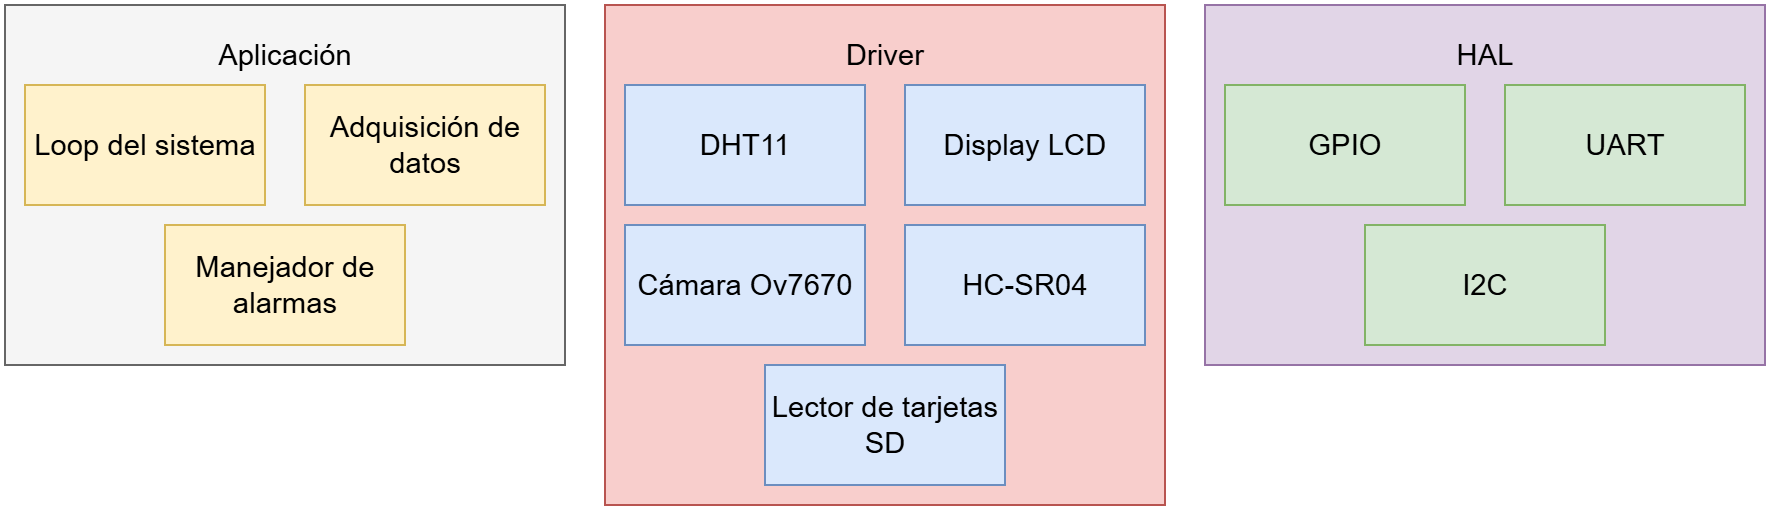
\includegraphics[width=1\textwidth, height=0.29\textheight]{./Figures/firmware_general.png}
	\caption{Capas del firmware.}
	\label{fig:firmware_general}
\end{figure}

\vspace{1cm}

\subsubsection{Capa HAL}

La capa HAL (\textit{Hardware Abstraction Layer}), proporcionada por el fabricante del microcontrolador, representa el nivel más bajo del sistema y permite que las capas superiores interactúen con los periféricos del microcontrolador a través de funciones en lenguaje C. Esta capa abstrae las complejidades del hardware y facilita el acceso a las funcionalidades del microcontrolador, lo que mejora la eficiencia y modularidad del sistema. A continuación, se describen los módulos clave de la capa HAL utilizados en el firmware:

\begin{itemize}
\item GPIO (\textit{General Purpose Input/Output}): proporciona funciones para el manejo de las entradas y salidas digitales del microcontrolador. En este sistema, la capa de aplicación utiliza las funciones GPIO para gestionar los indicadores LED de depuración y controlar el encendido y reinicio del sistema. Estos elementos resultan fundamentales para verificar el correcto funcionamiento y estado del nodo sensor en tiempo real.
\item UART (\textit{Universal Asynchronous Receiver-Transmitter}): brinda funciones específicas para la lectura y escritura del puerto UART del microcontrolador, lo que permite la comunicación en serie. El firmware emplea estas funciones UART para establecer un enlace con módulos adicionales, lo que facilita la transmisión de datos sin la necesidad de un reloj compartido. Esta característica es esencial para intercambiar información de manera confiable entre los componentes del sistema.
\item I2C (\textit{Inter-Integrated Circuit}): proporciona funciones para la transmisión y recepción de datos mediante el protocolo I2C, que permite la comunicación con dispositivos externos. En este proyecto, el driver de la pantalla LCD utiliza el protocolo I2C para actualizar la visualización de datos en tiempo real. La implementación del protocolo I2C permite una integración flexible y eficaz de dispositivos adicionales, lo que mejora la interacción entre los distintos módulos del sistema.
\end{itemize}

\subsubsection{Capa drivers}
\label{Capa_drivers}

La capa de drivers, o manejadores de dispositivos, consiste en los controladores desarrollados para facilitar la interacción entre el microcontrolador y el hardware externo. Cada driver se compone de funciones especializadas que permiten el control y gestión de dispositivos específicos. A continuación, se describen los drivers implementados para cada componente del sistema:

Driver de la cámara Ov7670: este controlador permite gestionar la captura de imágenes y configuración de la cámara. Entre sus funciones se incluyen:
\begin{itemize}
\item Iniciar captura de imagen: activa la adquisición de imágenes desde la cámara.
\item Detener captura de imagen: interrumpe el proceso de captura.
\item Pausar captura de imagen: suspende temporalmente la captura de imágenes sin perder la configuración actual.
\item Reanudar captura de imagen: retoma la captura desde el estado pausado.
\item Cambiar la resolución de captura de imagen: ajusta la resolución de imagen para adaptarse a los requisitos del sistema y a las condiciones de operación.
\end{itemize}

Driver para el sensor de temperatura y humedad DHT11: este controlador facilita la adquisición de datos ambientales y ofrece funciones clave para obtener y procesar las lecturas de temperatura y humedad. Las funcionalidades incluidas son:
\begin{itemize}
\item Tomar temperatura: obtiene la temperatura del entorno desde el sensor.
\item Tomar humedad: adquiere el nivel de humedad ambiente.
\item Devolver la temperatura en grados Celsius: convierte y presenta la temperatura en la escala Celsius.
\item Devolver la temperatura en grados Fahrenheit: convierte y muestra la temperatura en la escala Fahrenheit.
\end{itemize}

Driver del sensor ultrasónico HC-SR04: este controlador permite medir la distancia entre el sensor y los objetos cercanos mediante pulsos ultrasónicos. Sus funciones principales son:
\begin{itemize}
\item Enviar señal de eco: emite una señal ultrasónica hacia el objeto.
\item Calcular distancia en centímetros: calcula y devuelve la distancia medida en centímetros.
\item Calcular distancia en metros: calcula y retorna la distancia medida en metros.
\item Detener la señal de eco: interrumpe la emisión de pulsos ultrasónicos.
\end{itemize}

Driver para la pantalla LCD: este controlador gestiona la visualización de datos en la pantalla LCD y ofrece al operador información en tiempo real sobre el estado del sistema. Entre las funciones disponibles se encuentran:
\begin{itemize}
\item Refrescar pantalla: actualiza la información mostrada en la pantalla para reflejar los datos más recientes.
\item Mostrar mensaje en pantalla: presenta un mensaje específico en la pantalla para el usuario.
\item Limpiar pantalla: borra el contenido actual en la pantalla.
\item Escribir al comienzo de la línea: permite escribir texto desde el inicio de una línea específica.
\item Escribir al final de la línea: escribe texto en la posición final de una línea seleccionada.
\end{itemize}

Driver del lector de tarjetas SD: este controlador permite el almacenamiento seguro y organizado de los datos capturados en una tarjeta SD. Las funciones que incluye son:
\begin{itemize}
\item Escribir en la tarjeta: graba datos en la tarjeta SD para su posterior análisis.
\item Borrar contenido de la tarjeta: elimina los archivos almacenados en la tarjeta.
\item Comprobar espacio en la tarjeta: verifica el espacio libre disponible en la tarjeta SD.
\item Comprobar formateo de la tarjeta: asegura que la tarjeta esté correctamente formateada para evitar errores de lectura/escritura.
\end{itemize}

\subsubsection{Capa aplicación}
\label{capa_aplicacion}

La capa de aplicación representa el nivel jerárquico superior del sistema y se implementó sobre el sistema operativo en tiempo real FreeRTOS, lo que permite una mayor escalabilidad del código. Esta capa coordina y organiza la lógica de las funciones avanzadas del sistema mediante tres tareas principales, descritas a continuación:

\begin{itemize}
\item Loop del sistema: esta tarea proporciona la secuencialidad necesaria para que el sistema funcione de manera continua y ordenada. Actúa como el “hilo conductor” de todas las operaciones, que gestiona el flujo de actividades y garantiza que cada módulo cumpla su función en el momento oportuno.
\item Adquisición de datos: responsable de leer los datos provenientes de cada sensor, esta tarea asegura que el sistema capture información ambiental y visual de manera constante y precisa. Además, coordina las peticiones de cada sensor para evitar conflictos y optimizar el uso de recursos, lo que permite que la información esté lista para su posterior procesamiento y análisis.
\item Manejador de alarmas: esta tarea supervisa las condiciones críticas del sistema, como alertas ante eventos de desconexión en los dispositivos o falta de memoria. El manejador de alarmas proporciona una capa de seguridad adicional, que alerta sobre posibles problemas de funcionamiento y evitar fallos en el sistema.
\end{itemize}

\subsection{Nodo detector de objetos}

El nodo detector de objetos es el componente encargado de analizar las imágenes adquiridas por el nodo sensor. Este se basa en técnicas de visión por computadora y aprendizaje automático, tiene la capacidad de identificar y contar los frutos presentes en las imágenes. 

ME FALTA AMPLIAR Y DESARROLLAR. VOY A PONER IMAGEN DE NODO DETECTOR DE OBJETOS.

\section{Arquitectura del firmware}

La arquitectura del firmware del sistema está diseñada para optimizar la coordinación y el control de múltiples componentes, lo que asegura una operación eficiente y una respuesta rápida a eventos internos y externos. Se implementaron dos patrones arquitectónicos principales: el patrón de observar y reaccionar y el de segmentación de procesos, cada uno de ellos cumple funciones específicas dentro de la estructura del firmware.

\subsection{Patrón de observar y reaccionar}

Este patrón mostrado en la figura \ref{fig:patron_de_observar_y_reaccionar} permite que el sistema responda de inmediato a cambios en el entorno o en los estados de los componentes. En la práctica, cada módulo del firmware permanece en constante monitoreo de las señales y datos provenientes de los sensores y dispositivos externos, como el sensor de temperatura y humedad, el sensor ultrasónico y la cámara. 

En el momento que alguno de estos dispositivos genera un cambio relevante en sus lecturas (por ejemplo, una variación de temperatura o una nueva imagen capturada), el sistema ``observa'' esta alteración y automáticamente ``reacciona'' para ejecutar las acciones correspondientes, como almacenar los datos en la SD o actualizar la pantalla LCD. 

Este enfoque facilita una respuesta inmediata a los eventos sin la necesidad de que el sistema esté en modo de consulta continua, esto optimiza el uso de los recursos y reduce la latencia en la toma de decisiones.

\vspace{1cm}
\begin{figure}[htbp]
	\centering
	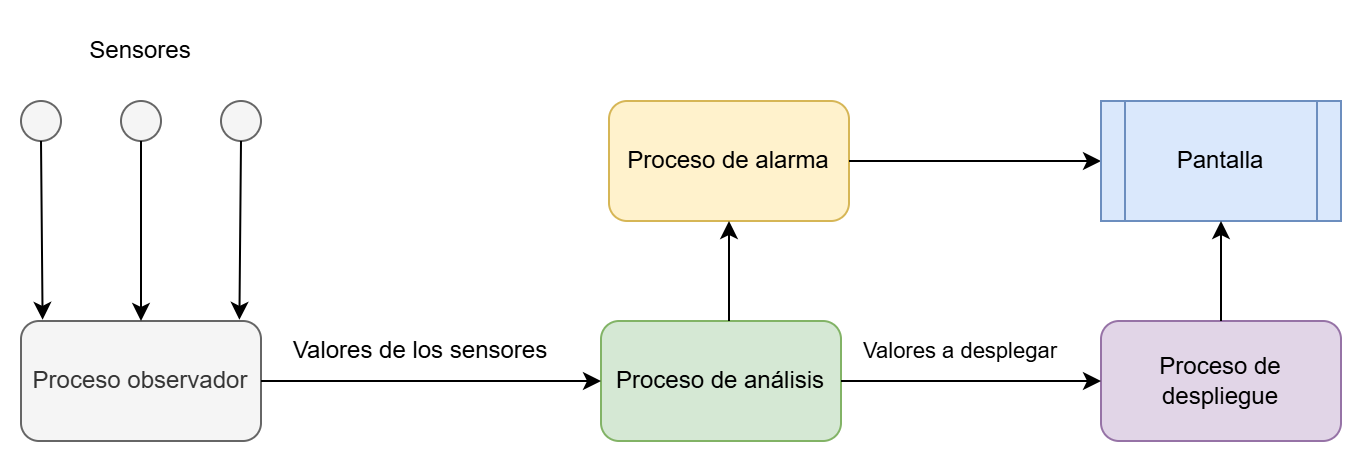
\includegraphics[width=0.9\textwidth, height=0.25\textheight]{./Figures/patron_de_observar_y_reaccionar.png}
	\caption{Patrón de observar y reaccionar.}
	\label{fig:patron_de_observar_y_reaccionar}
\end{figure}
\vspace{1cm}

\subsection{Patrón de segmentación de procesos}

Este patrón mostrado en la figura \ref{fig:segmentacion_de_procesos} se utiliza para transformar los datos obtenidos de los sensores, convirtiéndolos de su formato original a una representación adecuada antes de que puedan ser procesados eficazmente. 

Al realizar esta transformación inicial, el sistema asegura que los datos se presenten de manera uniforme y comprensible, lo que optimiza la precisión y consistencia en las etapas posteriores de procesamiento. Por ejemplo, los valores crudos obtenidos del sensor de temperatura pueden ser transformados en grados Celsius o Fahrenheit según las necesidades del sistema, y los datos del sensor ultrasónico se convierten en metros o centímetros. 

Esta normalización facilita que otros módulos del firmware interpreten los datos de manera rápida y sin ambigüedades, en consecuencia permite una respuesta más eficiente y coherente en la operación del sistema.

\vspace{1cm}
\begin{figure}[htbp]
	\centering
	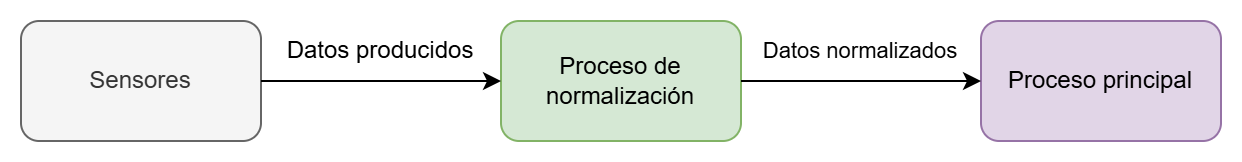
\includegraphics[width=0.9\textwidth, height=0.1\textheight]{./Figures/segmentacion_de_procesos.png}
	\caption{Segmentación de procesos.}
	\label{fig:segmentacion_de_procesos}
\end{figure}
\vspace{1cm}

\section{Módulos del firmware}

Los módulos están organizados en el firmware como funciones independientes que operan de forma coordinada y autónoma. Al segmentar el procesamiento, el firmware asigna tareas específicas a cada módulo, lo que permite que funcionen de manera paralela y reducir el riesgo de interferencias entre procesos. Así, tareas como la captura de imágenes, el monitoreo ambiental y el manejo de la interfaz de usuario pueden ejecutarse sin interrupciones.

Además, la segmentación facilita la escalabilidad del firmware, ya que los módulos pueden ser modificados o ampliados sin afectar la arquitectura completa, lo que permite agregar nuevos dispositivos o mejorar funcionalidades en futuras versiones del sistema. Cada módulo mostrado en la figura \ref{fig:modulos_del_firmware} representa a los drivers mencionados en la sección \ref{Capa_drivers}.

Los módulos operan de manera estructurada y siguen una secuencia de pasos específicos para procesar y distribuir la información capturada por el sistema:

\vspace{1cm}
\begin{figure}[htbp]
	\centering
	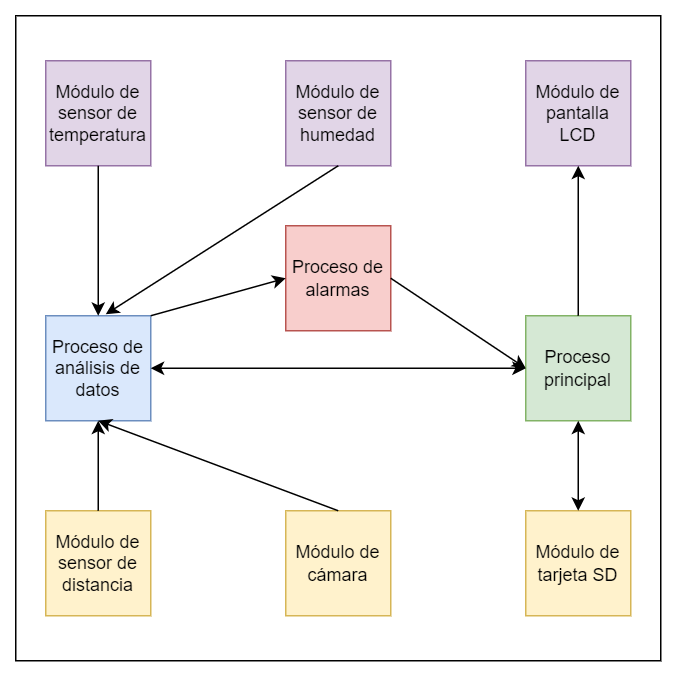
\includegraphics[width=0.9\textwidth, height=0.5\textheight]{./Figures/modulos_del_firmware.png}
	\caption{Módulos del firmware.}
	\label{fig:modulos_del_firmware}
\end{figure}
\vspace{1cm}

\begin{itemize}
\item Módulo de sensor de temperatura: recibe los datos de temperatura directamente del sensor y los transfiere al proceso de análisis de datos para su interpretación y uso en el sistema.
\item Módulo de sensor de humedad: recolecta las lecturas de humedad y las dirige al proceso de análisis de datos, donde estas mediciones contribuyen a la evaluación del entorno del sistema.
\item Monitor de sensor de distancia: captura los datos del sensor de distancia y los envía al proceso de análisis de datos, lo que permite la verificación de la proximidad de los objetos capturados por la cámara.
\item Módulo de pantalla LCD: asegura que la información generada por el sistema, incluidos los datos de sensores y el estado operativo, se muestre correctamente en el display, lo que proporciona al usuario una visión clara y accesible.
\item Módulo de tarjeta SD: gestiona el almacenamiento permanente de datos en la tarjeta SD, al recibir la información ya procesada desde el proceso principal. Si el sistema lo requiere, puede consultar la memoria para recuperar datos históricos y los transfiere de vuelta al proceso principal.
\item Módulo de cámara: realiza las capturas de imagen y las dirige al proceso de análisis de datos, donde se realiza el procesamiento visual o cualquier análisis relevante que se integre a los cálculos generales.
\item Proceso de análisis de datos: procesa los datos obtenidos por los sensores, lo que genera los cálculos necesarios para obtener parámetros clave del entorno. Una vez procesados, envía estos resultados al proceso principal o, si se detecta algún valor fuera de lo normal, lo comunica directamente al proceso de alarmas.
\item Proceso de alarmas: recibe las alertas generadas por el proceso de análisis de datos al detectar valores anómalos. Luego las envía al proceso principal para su gestión.
\item Proceso principal: coordina el sistema central, para gestionar la solicitud y envío de datos al módulo de almacenamiento en la tarjeta SD y transfiere los resultados relevantes al módulo de pantalla LCD, lo que mantiene una interacción eficiente y fluida entre los componentes.
\end{itemize}

\section{Desarrollo del firmware}

Para el desarrollo del firmware se empleó STM32CubeIDE, el entorno de desarrollo integrado (IDE) oficial proporcionado por STMicroelectronics. Este IDE ofrece un conjunto de herramientas y bibliotecas diseñadas específicamente para facilitar el trabajo con microcontroladores de la serie STM32. 

El firmware se implementó sobre FreeRTOS, un sistema operativo en tiempo real ampliamente utilizado en sistemas embebidos. En este desarrollo se integraron varias de las funcionalidades de FreeRTOS, como las colas para la transferencia ordenada de datos entre tareas, los semáforos para la sincronización entre procesos, y el uso de tareas específicas para segmentar las funciones del firmware. Además, se configuraron diversas interrupciones que permiten al sistema reaccionar instantáneamente ante eventos externos, como la llegada de datos de un sensor o la detección de un cambio en el entorno de trabajo.

Este diseño modular del firmware permite la implementación de colas y semáforos, el sistema logra una comunicación eficiente entre sus distintos módulos, lo que mantiene la integridad de los datos y evitar bloqueos o conflictos en el flujo de información.

En la Figura \ref{fig:DdF_firmware} se presenta un diagrama de flujo que describe el proceso de inicialización del firmware. Este diagrama ilustra cada uno de los pasos que el sistema sigue desde el inicio, luego por la configuración de los periféricos y la inicialización de las tareas del sistema, hasta el punto en que el firmware queda listo para operar. La organización detallada del flujo de inicialización asegura que cada módulo y sensor del nodo funcione correctamente y en el orden adecuado, lo que garantiza una estabilidad y eficiencia del sistema durante su funcionamiento.

\vspace{1cm}
\begin{figure}[htbp]
	\centering
	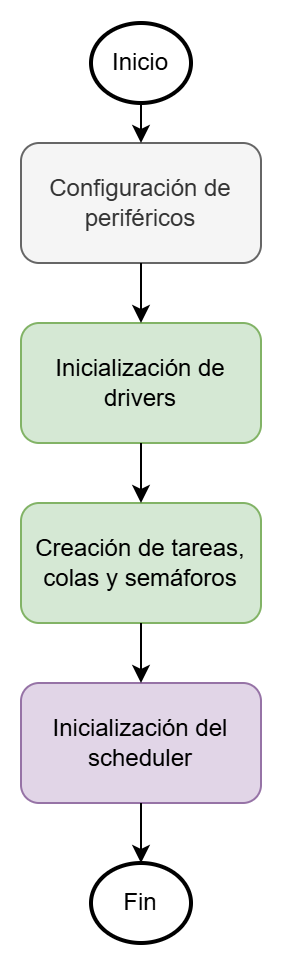
\includegraphics[width=0.3\textwidth, height=0.6\textheight]{./Figures/DdF_firmware.png}
	\caption{Diagrama de flujo de inicialización del firmware.}
	\label{fig:DdF_firmware}
\end{figure}
\vspace{1cm}

Para el control del sistema se crearon dos tareas sobre FreeRTOS, que se comunican
y se sincronizan a través de colas y semáforos.

\subsection{Tarea adquisición de datos}

La tarea de adquisición de datos cumple un rol esencial en la obtención de las lecturas de los sensores y en la garantía de un flujo continuo y preciso de información hacia el sistema. Esta tarea sigue un flujo estructurado, mostrado en el diagrama de flujo de la Figura \ref{fig:DdF_tarea_adquisición_datos}, donde cada paso asegura que los datos sean recogidos y procesados de manera eficiente.

\vspace{1cm}
\begin{figure}[htbp]
	\centering
	\includegraphics[width=0.45\textwidth, height=0.45\textheight]{./Figures/DdF_tarea_adquisición_datos.png}
	\caption{Diagrama de flujo tarea de adquisición de datos.}
	\label{fig:DdF_tarea_adquisición_datos}
\end{figure}
\vspace{1cm}

El proceso de adquisición comienza con la verificación de la cola de adquisición para detectar si existen solicitudes pendientes de datos. Si la cola contiene datos, la tarea procede a iniciar la lectura de todos los sensores del sistema. Estos datos, una vez adquiridos, se colocan en la cola de datos y alarmas, lo que permite que otros procesos, como el análisis y las alarmas, accedan a la información en tiempo real.

En caso de que la cola de adquisición esté vacía, la tarea de adquisición de datos se bloquea temporalmente para optimizar el uso de recursos, al permanecer en espera hasta que una nueva solicitud sea recibida en la cola. Esta capacidad de bloqueo y activación automática asegura que el sistema mantenga su eficiencia y libere recursos en el momento que no se requiera una lectura inmediata, además de garantizar que los datos recogidos sean siempre actuales.

Cada vez que los valores leídos presentan variaciones significativas o caen fuera de los rangos normales, el sistema de alarmas puede actuar en función de estos datos y enviar una alerta al proceso de alarmas, que luego gestiona la respuesta adecuada en el sistema.

\subsection{Tarea manejador de alarmas}

El manejador de alarmas supervisa los valores de los sensores para asegurar que se mantengan dentro de los límites permitidos de cada variable. En caso de detectar algún valor fuera de los parámetros establecidos, activa una alarma para alertar al sistema. El diagrama de flujo de esta tarea puede observarse en la Figura \ref{fig:DdF_tarea_manejador_alarmas}.

\vspace{1cm}
\begin{figure}[htbp]
	\centering
	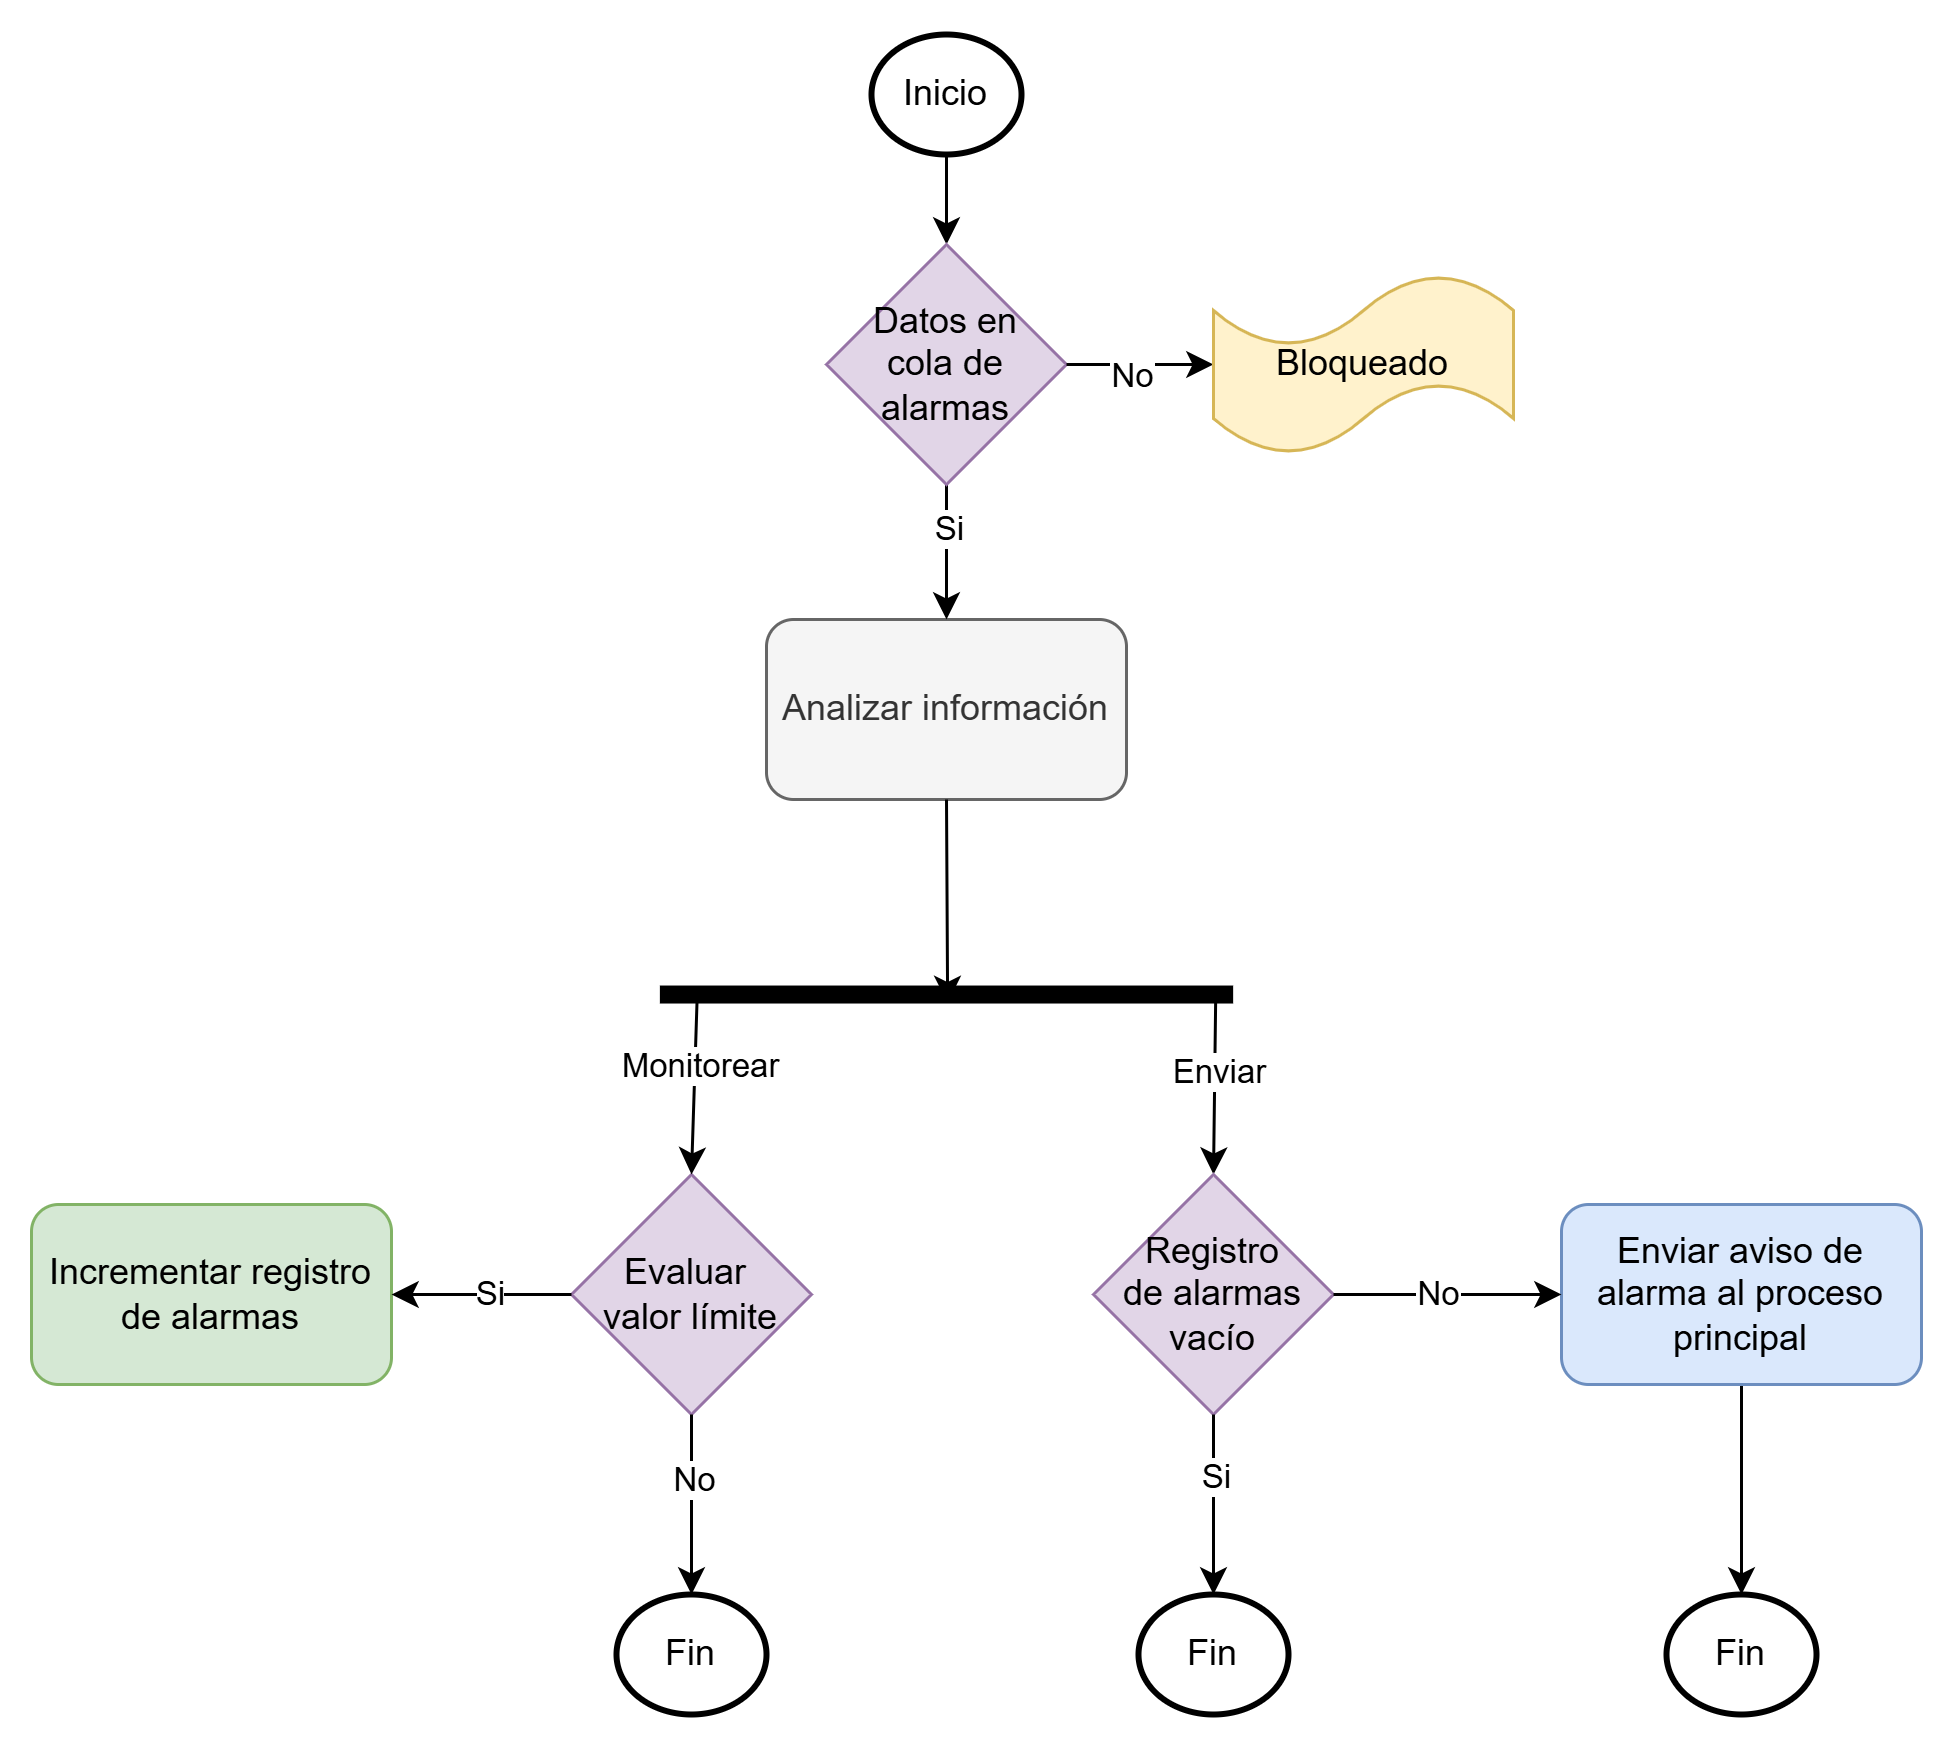
\includegraphics[width=1.0\textwidth, height=0.6\textheight]{./Figures/DdF_tarea_manejador_alarmas.png}
	\caption{Diagrama de flujo de la tarea manejadora de alarmas.}
	\label{fig:DdF_tarea_manejador_alarmas}
\end{figure}
\vspace{1cm}

Al comenzar el bucle infinito de monitoreo, el manejador inspecciona de manera constante la cola de alarmas en busca de eventos. Si se encuentran datos en esta cola, analiza la información recibida, que puede indicar dos tipos de eventos: monitorear y enviar.

\begin{itemize}
\item Evento monitorear: verifica si el valor de cada sensor cae por debajo o excede los valores de límite previamente definidos para cada variable. Si alguno de estos valores infringe los límites, se incrementa una variable que registra la cantidad de alarmas activas en el sistema. Esta información resulta fundamental para monitorear el estado del sistema en tiempo real y detectar situaciones de riesgo de manera inmediata.
\item Evento enviar: se verifica si existen alarmas activas en el sistema. En caso afirmativo, notifica al proceso principal para que ejecute las acciones necesarias, como activar una alerta visual. Esta comunicación garantiza una respuesta rápida y adecuada ante cualquier situación crítica detectada.
\end{itemize}

En el momento que no se encuentren datos en la cola de alarmas, la tarea entra en un estado de bloqueo. Esto optimiza el uso de recursos y detiene temporalmente la ejecución hasta que se recibe un nuevo dato. Esta estructura permite que el sistema opere de manera eficiente, ya que reacciona solo ante anomalías y no consume recursos innecesarios en condiciones normales.


% Chapter Template

\chapter{Ensayos y resultados} % Main chapter title

\label{Chapter4} % Change X to a consecutive number; for referencing this chapter elsewhere, use \ref{ChapterX}
En este capítulo se describen las pruebas realizadas para validar el hardware y software desarrollados. Se utilizaron herramientas de automatización de pruebas y hardware externo. Esto permitió contrastar y analizar los datos capturados por cada sensor, con el objetivo de verificar la precisión y robustez del sistema.

%----------------------------------------------------------------------------------------
%	SECTION 1
%----------------------------------------------------------------------------------------

\section{Pruebas unitarias del firmware}
\label{sec:pruebas_unitarias}

En esta sección se presentan pruebas unitarias para validar las funcionalidades clave del software, lo que asegura la precisión y estabilidad de cada componente. Durante la implementación de los drivers, se aplicó la metodología de desarrollo Test-Driven Development (TDD) \citep{ieee2023}.

Esta metodología establece la creación de pruebas unitarias antes de cada módulo y garantiza que el código cumpla con los requerimientos especificados desde las primeras etapas.

Para el desarrollo de pruebas automáticas, se empleó Ceedling, una herramienta robusta que facilitó la creación, ejecución y gestión de pruebas, lo que asegura una verificación consistente de cada funcionalidad.

\subsection{Prueba de cámara Ov7670}

La validación del driver de la cámara Ov7670 fue fundamental para garantizar que el sistema capturara imágenes con precisión y fiabilidad, al cumplir los requisitos en términos de resolución y capacidad de captura en tiempo real.

La prueba incluyó aspectos clave, como la inicialización de la cámara, la captura de imágenes en diferentes resoluciones y la transmisión de datos al proceso principal para su almacenamiento y análisis.

Durante las pruebas, se evaluaron distintas configuraciones de la cámara Ov7670, para verificar los ajustes de resolución y formato de imagen. La cobertura obtenida en las pruebas reflejó la capacidad del driver para mantener la estabilidad y calidad en la captura de imágenes incluso en condiciones de carga intensa. Además, los informes de prueba permitieron identificar y solucionar fallas menores, como errores en la sincronización del módulo de captura o posibles pérdidas de datos en resoluciones altas, lo que asegura un flujo constante y sin interrupciones. La figura \ref{fig:test_ov7670_camera}
muestra los resultados de las pruebas realizadas.

Otro aspecto evaluado fue la integración del driver con el sistema general. Este proceso resultó crucial para validar la robustez del sistema ante interrupciones inesperadas.

\vspace{1cm}

\begin{figure}[htbp]
	\centering
	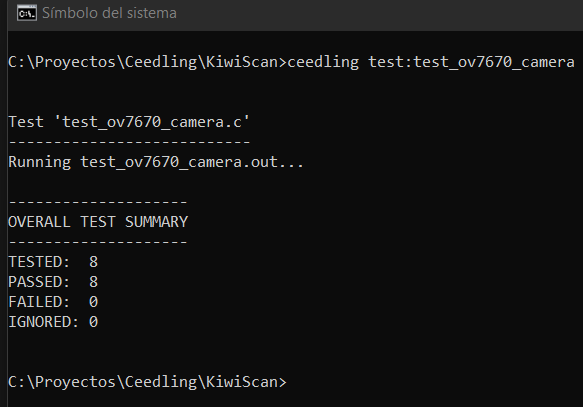
\includegraphics[width=0.7\textwidth, height=0.3\textheight]{./Figures/test_ov7670_camera.png}
	\caption{Test realizado a la cámara Ov7670.}
	\label{fig:test_ov7670_camera}
\end{figure}

\vspace{1cm}

\subsection{Prueba del sensor ultrasónico HC-SR04}

El proceso de prueba abarcó varias funciones clave del driver, como la inicialización del sensor, el envío de pulsos de activación, y la recepción y procesamiento de los ecos de respuesta que miden la distancia. Ceedling ejecutó pruebas unitarias para cada una de estas funciones, lo que generó informes detallados sobre la precisión y consistencia de los resultados. Este enfoque garantizó que el sensor ofreciera mediciones confiables y respondiera adecuadamente ante diferentes distancias, desde rangos cortos hasta los límites efectivos del sensor.

Otra área de prueba clave fue la integración del sensor con el sistema general y la manera en que el driver del HC-SR04 gestionaba las interrupciones durante la medición de distancias. Esta verificación fue esencial para confirmar que el sistema mantuviera un flujo de datos continuo.

Finalmente, se realizaron pruebas para analizar el manejo de errores en el driver, especialmente en situaciones en las que el sensor no recibía respuesta de eco o detectaba obstrucciones inesperadas. Se validó que el sistema reaccionara correctamente ante estas situaciones. La figura \ref{fig:test_hc_sr04_sensor} muestra los resultados de las pruebas realizadas.

\vspace{1cm}

\begin{figure}[htbp]
	\centering
	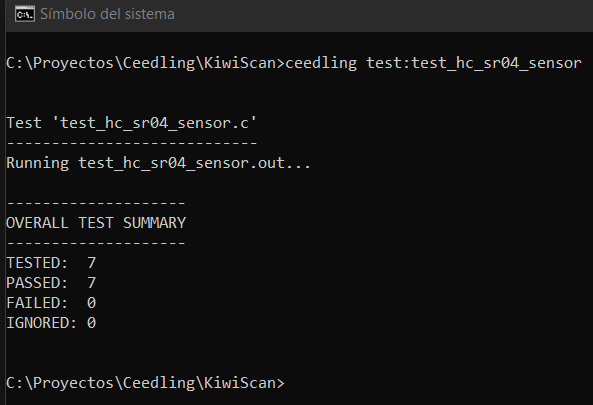
\includegraphics[width=0.7\textwidth, height=0.3\textheight]{./Figures/test_hc_sr04_sensor.png}
	\caption{Test realizado al sensor ultrasónico HC-SR04.}
	\label{fig:test_hc_sr04_sensor}
\end{figure}

\vspace{1cm}

\subsection{Prueba del lector de tarjetas SD}

Las pruebas iniciales evaluaron las operaciones de escritura y lectura, funciones esenciales para el almacenamiento continuo de datos capturados por los sensores. Cada operación fue probada con diferentes tamaños de archivos, para simular diversos escenarios de uso, desde pequeñas cantidades de datos hasta archivos de mayor tamaño, para determinar la capacidad del driver para manejar un flujo de datos sostenido. La figura \ref{fig:test_sd_card_reader} muestra los resultados de las pruebas realizadas.

\vspace{1cm}

\begin{figure}[htbp]
	\centering
	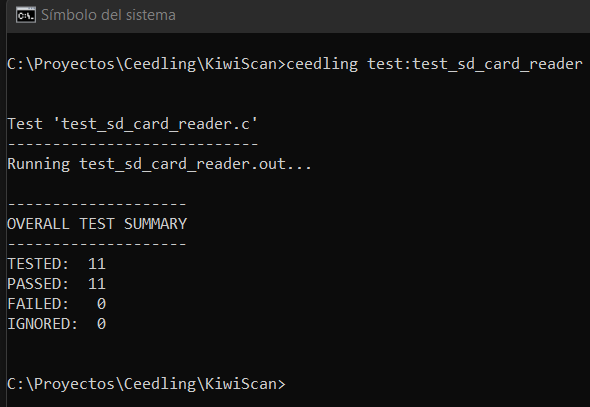
\includegraphics[width=0.7\textwidth, height=0.3\textheight]{./Figures/test_sd_card_reader.png}
	\caption{Test realizado al lector de tarjetas SD.}
	\label{fig:test_sd_card_reader}
\end{figure}

\vspace{1cm}

Además, se evaluaron las capacidades del driver para detectar y gestionar tarjetas SD con diferentes formatos. La lectura y escritura en tarjetas formateadas en sistemas FAT32 y exFAT permitió verificar la flexibilidad del driver y su compatibilidad con distintos tipos de almacenamiento. Este aspecto fue crítico, pues garantiza que el sistema se adapte a diversas tarjetas sin requerir reconfiguraciones manuales.

Se simularon problemas comunes, como la extracción inesperada de la tarjeta, errores en la escritura y fallos de inicialización. Esto permitió observar cómo el driver respondía ante estos problemas, para verificar que el sistema registrará la interrupción o emitiera alertas adecuadas sin comprometer la estabilidad del sistema.

\subsection{Prueba de integración de drivers}

La prueba de integración de drivers tuvo como objetivo evaluar el desempeño conjunto de los componentes desarrollados y comprobar su funcionamiento de manera coordinada y sin interferencias. Esta prueba incluyó los drivers del sensor de temperatura y humedad DHT11, el sensor ultrasónico HC-SR04, la cámara OV7670, el display LCD y el lector de tarjetas SD, los que operaron simultáneamente para asegurar una respuesta del sistema.

En el proceso, cada driver fue evaluado en condiciones similares a las de su operación final, para verificar la capacidad del sistema. Los resultados indicaron que todos los drivers se integraron correctamente, sin dificultades en los ensayos realizados, con una sincronización adecuada entre los distintos módulos. La figura \ref{fig:test_integrated_drivers} muestra los resultados obtenidos.

\vspace{1cm}

\begin{figure}[htbp]
	\centering
	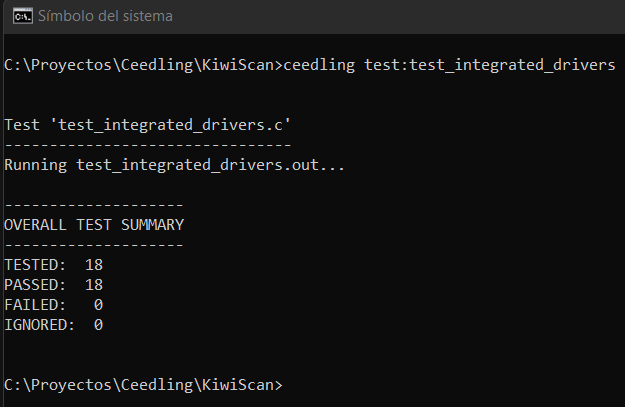
\includegraphics[width=0.7\textwidth, height=0.3\textheight]{./Figures/test_integrated_drivers.png}
	\caption{Test de integración de drivers.}
	\label{fig:test_integrated_drivers}
\end{figure}

\vspace{1cm}

Las pruebas confirmaron que el sistema responde adecuadamente a las demandas de funcionamiento en conjunto, sin comprometer la velocidad ni la precisión de las mediciones y salidas visuales.

\section{Pruebas funcionales del hardware}
\label{pruebas_funcionales_hardware}

Esta sección expone los ensayos realizados para evaluar la precisión y confiabilidad de los sensores integrados en el sistema. El propósito principal es contrastar las mediciones del sensor de temperatura y humedad DHT11, el sensor ultrasónico HC-SR04 y la cámara Ov7670 con las obtenidas por otros dispositivos o herramientas.

\subsection{Evaluación de precisión en temperatura y humedad del sensor DHT11}

Para determinar la precisión del sensor DHT11 en la medición de temperatura y humedad, se realizaron pruebas comparativas con un termómetro higrómetro de laboratorio como referencia. Esta prueba tuvo lugar durante un periodo de dos horas, con mediciones cada 15 minutos a partir del mediodía. La prueba se llevó a cabo en un entorno controlado, con una temperatura base aproximada de 25 ° C.

En cada intervalo de tiempo, se registraron los datos de temperatura y humedad captados por ambos dispositivos, lo que permitió identificar las diferencias entre el sensor DHT11 y el termómetro higrómetro. Se observó que el DHT11 reportó variaciones de entre 1 y 2 puntos respecto a la referencia de laboratorio, tanto en temperatura como en humedad, lo que muestra una desviación mínima. Los resultados de esta comparación se presentan en la tabla \ref{tab:DHT11_comparacion}.

\vspace{1cm}

\begin{table}[h]
    \centering
    \caption[Comparación de mediciones de temperatura y humedad]{Comparación de mediciones de temperatura y humedad.}
    \begin{tabularx}{\textwidth}{l X X X X X X X}  % Cambia el ancho de la última columna
        \toprule
        \textbf{Hora} & \textbf{Temp. DHT11} & \textbf{Temp. higrómetro} & \textbf{Dif. temp.} & \textbf{Hum. DHT11} & \textbf{Hum. higrómetro} & \textbf{Dif. hum.} \\
        \midrule
        12:00 PM & 25.5 & 25.0 & +0.5 & 47 & 49 & -2\\		
        12:15 PM & 26.0 & 25.5 & +0.5 & 46 & 48	& -2\\
        12:30 PM & 26.3 & 26.0 & +0.3 & 48 & 49 & -1\\
        12:45 PM & 26.5 & 26.2 & +0.3 & 49 & 50 & -1\\
        01:00 PM & 26.7 & 26.5 & +0.2 & 50 & 52 & -2\\
        01:15 PM & 27.0 & 26.8 & +0.2 & 51 & 53 & -2\\
        01:30 PM & 27.2 & 27.0 & +0.2 & 52 & 54 & -2\\
        01:45 PM & 27.3 & 27.1 & +0.2 & 52 & 54 & -2\\
        02:00 PM & 27.5 & 27.3 & +0.2 & 53 & 55 & -2\\
        \bottomrule
    \end{tabularx}
    \label{tab:DHT11_comparacion}
\end{table}

\vspace{1cm}

\subsection{Análisis de precisión en medición de distancia con el sensor ultrasónico HC-SR04}

El objetivo de esta prueba fue evaluar la precisión del sensor ultrasónico HC-SR04 en la medición de distancias. Se establecieron seis puntos de referencia a distintas distancias de una muestra de una planta de kiwi: 50 centímetros, 1 metro, 1.5 metros, 2 metros, 2.5 metros y 3 metros. Las mediciones de referencia se obtuvieron con una cinta métrica convencional, y luego se registraron las lecturas del sensor HC-SR04 para cada posición.

Los resultados evidencian que el sensor HC-SR04 presenta una gran precisión en distancias cortas, al calcular sin errores la medida de 50 centímetros. Sin embargo, conforme aumenta la distancia, se observan diferencias leves que van de 1 a 5 centímetros en comparación con la referencia. Estos datos demuestran que el sensor es bastante preciso en rangos de hasta un metro y mantiene una tolerancia aceptable para aplicaciones de detección de distancias mayores. La tabla \ref{tab:HCSR04_comparacion} resume las mediciones obtenidas.

\vspace{1cm}

\begin{table}[h]
	\centering
	\caption[Comparación de mediciones tomadas]{Comparación de mediciones tomadas.}
	\begin{tabular}{c c c}    
		\toprule
		\textbf{Distancia de referencia (cm)} 	 & \textbf{Medición del HC-SR04 (cm)} 		& \textbf{Diferencia (cm)}  \\
		\midrule
		50 & 50 & 0 \\		
		100 & 101 & +1 \\	
		150 & 151 & +1 \\	
            200 & 202 & +2 \\	
            250 & 253 & +3 \\	
            300 & 305 & +5 \\	
		\bottomrule
		\hline
	\end{tabular}
	\label{tab:HCSR04_comparacion}
\end{table}

\vspace{1cm}



% Chapter Template

\chapter{Conclusiones} % Main chapter title

\label{Chapter5} % Change X to a consecutive number; for referencing this chapter elsewhere, use \ref{ChapterX}
Todos los capítulos deben comenzar con un breve párrafo introductorio que indique cuál es el contenido que se encontrará al leerlo.  La redacción sobre el contenido de la memoria debe hacerse en presente y todo lo referido al proyecto en pasado, siempre de modo impersonal.


%----------------------------------------------------------------------------------------

%----------------------------------------------------------------------------------------
%	SECTION 1
%----------------------------------------------------------------------------------------

\section{Conclusiones generales }

La idea de esta sección es resaltar cuáles son los principales aportes del trabajo realizado y cómo se podría continuar. Debe ser especialmente breve y concisa. Es buena idea usar un listado para enumerar los logros obtenidos.

En esta sección no se deben incluir ni tablas ni gráficos.

Algunas preguntas que pueden servir para completar este capítulo:

\begin{itemize}
\item ¿Cuál es el grado de cumplimiento de los requerimientos?
\item ¿Cuán fielmente se puedo seguir la planificación original (cronograma incluido)?
\item ¿Se manifestó algunos de los riesgos identificados en la planificación? ¿Fue efectivo el plan de mitigación? ¿Se debió aplicar alguna otra acción no contemplada previamente?
\item Si se debieron hacer modificaciones a lo planificado ¿Cuáles fueron las causas y los efectos?
\item ¿Qué técnicas resultaron útiles para el desarrollo del proyecto y cuáles no tanto?
\end{itemize}


%----------------------------------------------------------------------------------------
%	SECTION 2
%----------------------------------------------------------------------------------------
\section{Próximos pasos}

Acá se indica cómo se podría continuar el trabajo más adelante.


%----------------------------------------------------------------------------------------
% Apéndices
%----------------------------------------------------------------------------------------

\appendix

% Incluir apéndices desde archivos separados si es necesario
%% Appendix A

\chapter{Appendix Title Here} % Main appendix title

\label{AppendixA} % For referencing this appendix elsewhere, use \ref{AppendixA}

Write your Appendix content here.

%----------------------------------------------------------------------------------------
% Bibliografía
%----------------------------------------------------------------------------------------

\renewcommand{\bibname}{Bibliografía} % Para asegurarte de que el título sea correcto
\phantomsection % Necesario para que el enlace del marcador sea correcto

\printbibliography[heading=bibintoc]

\end{document}






